\documentclass[11pt]{article}
\usepackage[margin=1.1in]{geometry}
\usepackage{amsmath,amssymb,amsthm}
\usepackage{graphicx}
\usepackage{booktabs}
\usepackage[hidelinks]{hyperref}

\newtheorem{theorem}{Theorem}
\newtheorem{proposition}{Proposition}
\newtheorem{lemma}{Lemma}
\newtheorem{corollary}{Corollary}
\theoremstyle{remark}
\newtheorem{remark}{Remark}

\newcommand{\R}{\mathbb{R}}
\newcommand{\E}{\mathbb{E}}
\newcommand{\Prob}{\mathbb{P}}

\title{The Runner-Up Principle for Counterfactual Races}
\author{Peter Cotton\thanks{Code, data, and machine verifications for every claim:
\url{https://github.com/microprediction/kinetics} (experiments 1, 7, 8, 10).
Web companion: \url{https://kinetics.microprediction.org}.}}
\date{August 2026 --- working draft}

\begin{document}
\maketitle

\begin{abstract}
Many systems reveal themselves only through races: $N$ latent processes compete, and
an observer records which one finished first. The natural counterfactual question ---
what happens if competitor $i$ is removed? --- turns out to be exactly nonidentified
from winner frequencies alone: the redistribution of the removed competitor's
probability is governed by a runner-up kernel $M$ on which winner data places no
constraint whatsoever. We give the sharp partial-identification set, and a data
hierarchy that resolves it: observing the runner-up identifies every single-deletion
counterfactual, and top-$(k{+}1)$ ranking prefixes identify every deletion of up to
$k$ competitors. A Markov substitution resolvent turns the runner-up kernel into
predictions for arbitrary blocked sets. We validate the hierarchy on real
first-passage physics --- Brownian narrow escape, where a truncation identity makes
one reflecting trajectory answer every blocked-set counterfactual exactly --- finding
that winner-only models degrade with deletion depth while the runner-up kernel
predicts at the sampling-noise floor, and that the substitution process is
empirically Markov. Finally, we show the kernel is not merely estimable but
\emph{computable}: Green-function hitting splits of the domain predict $M$ to within
sampling noise with no trajectory data, and the geometric kernel outperforms the
empirically measured one as an input to counterfactual prediction. Two practical
warnings emerge: the stationary encounter chain differs materially from the
first-transition kernel that counterfactuals require, and common time changes make
proportional-hazards (softmax) redistribution exact --- so deviations from it
measure differential structure only.
\end{abstract}

\section{Introduction}

A chemical system escapes a metastable state through one reaction channel out of
many; a stressed material fails at one bond; a diffusing particle is captured by one
of several boundary receptors; a bettor watches one horse win. In each case the
observable is the identity of the winner of a race among $N$ latent processes, and
in each case the operational questions are counterfactual: if this channel is
poisoned, this receptor blocked, this horse scratched --- where does its probability
go?

This paper is about what data can answer that question. The answer is organized by a
simple identity. Let $\pi$ denote the latent finishing order and
$p_i = \Prob(\pi_1 = i)$ the winner probabilities. If competitor $i$ is removed, the
winner is $j$ either because $j$ was going to win anyway, or because $i$ was going to
win with $j$ next best:
\begin{equation}
q_j^{(-i)} \;=\; p_j + p_i\, M_{ij},
\qquad
M_{ij} \;=\; \Prob(\pi_2 = j \mid \pi_1 = i).
\label{eq:runnerup}
\end{equation}
Everything about single deletions is carried by the \emph{runner-up kernel} $M$ ---
and, as Theorem~\ref{thm:nonid} states, winner data carries no information about $M$
at all. The identification failure is exact, not statistical, and it is the
finite-choice face of the classical nonidentifiability of competing risks
\cite{tsiatis1975,cox1959}. Its resolution is a data hierarchy
(Section~\ref{sec:hierarchy}): runner-up identities identify all single deletions;
$(k{+}1)$-prefixes identify all $\le k$-deletions; and a Markov substitution model
composes single-deletion knowledge into predictions for arbitrary blocked sets.

The paper's second half is empirical, on real first-passage physics. A
\emph{truncation identity} (Lemma~\ref{lem:trunc}) makes the Brownian narrow-escape
problem an ideal laboratory: one trajectory of the \emph{reflecting} process answers
every blocked-set counterfactual exactly, so a single simulation furnishes exact
ground truth for the entire deletion ensemble. On this testbed the hierarchy behaves
precisely as the theory predicts (Section~\ref{sec:experiments}), with a bonus: the
substitution process is empirically Markov, so pairs data alone matches full-prefix
accuracy at every tested deletion depth. Finally (Section~\ref{sec:geometry}) we
show the kernel is computable from the geometry of the domain --- Green-function
hitting splits --- to within the sampling noise of a $24{,}000$-trajectory
measurement, and that this geometric kernel is the \emph{best} available input to
counterfactual prediction, beating the empirical kernel it predicts.

Two cautions recur and deserve headline billing. First, the \emph{two-kernels
warning}: the stationary window-to-window encounter chain and the first-transition
kernel appearing in \eqref{eq:runnerup} differ by as much as $0.21$ in our
experiments, and counterfactuals want the latter; estimating $M$ from all
consecutive encounter pairs --- more data --- makes predictions \emph{worse}.
Second, the \emph{proportional-hazards normal form} (Lemma~\ref{lem:ph}): any common
time change of exponential clocks leaves the Luce/softmax redistribution law exact,
so observed deviations from proportional redistribution measure \emph{differential}
structure only. Both cautions are verified numerically in the companion repository,
as is every formula in this paper.

\paragraph{Related work.} The runner-up identity \eqref{eq:runnerup} is elementary
and surely folklore in fragments; our contribution is the sharp nonidentifiability
statement, the sufficiency hierarchy, and the physical program built on them. The
Markov substitution model of Section~\ref{sec:hierarchy} coincides in form with the
Markov-chain choice model of assortment optimization \cite{blanchet2016}; there it
is a modeling assumption fit to sales data, here it is derived semantics for
encounter processes, empirically validated and geometrically computable. Harville's
formula \cite{harville1973} and its position-discount descendants are completions of
winner data by an \emph{assumed} $M$; Thurstone \cite{thurstone1927} and Luce
\cite{luce1959} supply the classical latent-noise completions. The narrow-escape
literature \cite{holcman2014} provides the physical setting; competing-risks
nonidentifiability goes back to \cite{cox1959,tsiatis1975}. The fast lattice
transform used for the Thurstone baselines is from \cite{cotton2021}.

\section{Winner data does not identify deletions}

Let $S_N$ denote permutations of $\{1,\dots,N\}$ and let $P$ be any probability
distribution on $S_N$ (the law of the finishing order). Write $p_i = P(\pi_1 = i)$
and $M_{ij} = P(\pi_2 = j \mid \pi_1 = i)$ for $j \ne i$ (rows of $M$ are
probability vectors on $\{j \ne i\}$; set $M_{ii} = 0$).

\begin{theorem}[Winner-only nonidentifiability]\label{thm:nonid}
Let $p$ be any interior point of the simplex and $M$ any matrix with zero diagonal
and row sums one, $M_{ij} \ge 0$. Then there is a ranking distribution $P$ with
winner probabilities $p$ and runner-up kernel $M$.
\end{theorem}

\begin{proof}
Take $P(\pi) = p_{\pi_1} M_{\pi_1 \pi_2} / (N-2)!$\,. Summing over $\pi$:
$\sum_i p_i \sum_{j \ne i} M_{ij} = 1$, so $P$ is a probability distribution; its
winner marginal is $p$ and its runner-up kernel is $M$ by construction.
\end{proof}

\begin{corollary}[Sharp partial identification]\label{cor:polytope}
From winner probabilities alone, the single-deletion counterfactual is constrained
exactly to the polytope
\[
q_j^{(-i)} \in [\,p_j,\; p_j + p_i\,], \qquad \textstyle\sum_{j \ne i} q_j^{(-i)} = 1,
\]
and every point of it is attained.
\end{corollary}

The bounds are wide precisely where the question matters: deleting a strong
competitor ($p_i$ large) leaves its entire probability mass unallocated. Every
winner-only model in use --- proportional renormalization (Harville
\cite{harville1973}, equivalently Luce's axiom \cite{luce1959}), position discounts,
independent Thurstone completions --- selects a point of the polytope by assumption.
Such a completion can be \emph{useful}; Section~\ref{sec:experiments} measures how
useful, on physics that violates all of them. But it cannot be \emph{learned} from
the data it consumes, and Theorem~\ref{thm:nonid} says no cleverness will change
that.

One classical assumption deserves its own statement, because it is weaker than
usually presented, and because it calibrates what a violation means.

\begin{lemma}[Proportional-hazards normal form]\label{lem:ph}
Let the competitors' event times be independent with cumulative hazards
$H_i(t) = a_i H_0(t)$ for a common, arbitrary, increasing $H_0$. Then
$\Prob(i \text{ wins any subset race } A) = a_i / \sum_{j \in A} a_j$: the Luce law,
with proportional redistribution under deletion, holds exactly.
\end{lemma}

\begin{proof}
The time change $u = H_0(t)$ makes the times independent exponentials with rates
$a_i$, and the winner is unchanged by a common monotone time change.
\end{proof}

\begin{remark}
The lemma extends to \emph{randomly} modulated intensities
$\lambda_i(t) = a_i\,c(Y_t)$ driven by any common environment $Y$: conditional on
the path of $Y$ this is a common time change, so Luce holds at every mixing speed.
In the companion homogenization analysis (experiment 7 of the repository), the
first-order correction to Luce is a Green--Kubo functional of the intensity
covariances that vanishes identically for common-mode modulation --- verified to
$10^{-16}$. Deviations from proportional redistribution therefore measure
\emph{differential} loadings on the environment, never the environment's volatility
itself.
\end{remark}

\section{The data hierarchy and the substitution resolvent}\label{sec:hierarchy}

\begin{proposition}[Prefix sufficiency]\label{prop:prefix}
The law of the top-$(k{+}1)$ prefix $(\pi_1, \dots, \pi_{k+1})$ determines every
counterfactual winner distribution $q^{(-B)}$ with $|B| \le k$.
\end{proposition}

\begin{proof}
After blocking $B$, the winner is the first element of $\pi$ outside $B$, which
occupies one of the first $|B|+1$ positions; the event
$\{\text{winner after blocking } B \text{ is } j\}$ is measurable with respect to
the $(|B|+1)$-prefix.
\end{proof}

In particular, the runner-up identity \eqref{eq:runnerup} shows the $k=1$ case
explicitly, and the practical reading is the \emph{runner-up principle}: the
runner-up's identity is worth more, for deletion counterfactuals, than the winning
margin. A margin says how close the race was; it does not say where the winner's
probability goes.

For blocked sets of several competitors, single-deletion knowledge composes under a
Markov assumption on the substitution process. Let $M$ be a substitution kernel:
when demand (flux, probability) arrives at an unavailable competitor $i$, it moves
to $j$ with probability $M_{ij}$, repeating until it lands on an available one. Then
for available $A$ and blocked $B$,
\begin{equation}
q_A \;=\; p_A + p_B\,(I - M_{BB})^{-1} M_{BA}.
\label{eq:resolvent}
\end{equation}
The resolvent $(I - M_{BB})^{-1}$ sums substitution paths through the blocked set.
Formally this is the Markov-chain choice model of \cite{blanchet2016}; the content
here is that for encounter processes the kernel has independent meaning (next
distinct window hit), the Markov property is testable (and passes, below), and the
kernel is computable from geometry (Section~\ref{sec:geometry}).

\paragraph{The two-kernels warning.} An encounter process offers two natural
kernels: the \emph{first-transition} kernel --- the law of the second distinct
window given the first, starting from the system's actual initial condition ---
and the \emph{stationary encounter chain} --- transitions between consecutive
distinct windows along an infinite trajectory. They agree only if encounter
positions equilibrate between events. In the narrow-escape experiments below they
differ by up to $0.21$ in individual entries, and \eqref{eq:runnerup} unambiguously
wants the first-transition kernel: estimating $M$ from all consecutive encounter
pairs (which maximizes sample size) \emph{degrades} multi-block prediction. Data
hierarchies must name their kernel.

\section{Ranked narrow escape: the hierarchy on real physics}\label{sec:experiments}

\begin{lemma}[Truncation identity]\label{lem:trunc}
Let $X$ be a reflecting diffusion on a domain whose boundary contains disjoint
windows $W_1, \dots, W_N$, and let the encounter sequence be the ordered list of
distinct windows contacted by the path. For any subset $A$ made absorbing, the
absorbed process is the reflecting process stopped at its first $A$-encounter; in
particular, the winner under absorbing set $A$ is the first element of the
encounter sequence belonging to $A$.
\end{lemma}

\begin{proof}[Proof sketch]
Construct both processes from the same driving noise. Their paths coincide up to
the first $A$-contact, since reflection and absorption differ only on $A$, which
neither path has yet touched. \qedhere
\end{proof}

One reflecting trajectory therefore answers \emph{every} blocked-set counterfactual,
and a held-out batch of encounter sequences is exact ground truth for the entire
deletion ensemble simultaneously. (The identity was cross-checked against a direct
absorbing simulation: total-variation difference $0.012$ against a combined sampling
noise of $\approx 0.013$.)

\paragraph{Setup.} Brownian motion in the unit disk, $16$ disjoint boundary windows
of varied widths; $24{,}000$ reflecting trajectories, each recording its first $8$
distinct window encounters ($12{,}000$ for fitting, $12{,}000$ held out as truth);
$12$ random blocked sets of each size $1, 2, 3$. Models are scored by mean
total-variation distance between predicted and held-out counterfactual winner
distributions.

\begin{table}[h]
\centering
\begin{tabular}{lccc}
\toprule
model (data consumed) & singletons & pairs & triples \\
\midrule
Harville renormalization (winner only) & 0.0381 & 0.0570 & 0.0690 \\
independent Thurstone (winner only) & 0.0380 & 0.0562 & 0.0677 \\
runner-up kernel $M$ + resolvent \eqref{eq:resolvent} & \textbf{0.0154} & \textbf{0.0154} & \textbf{0.0160} \\
top-4 prefixes (direct evaluation) & 0.0154 & 0.0154 & 0.0157 \\
\bottomrule
\end{tabular}
\caption{Ranked narrow escape (geometry of experiment 8; sampling-noise floor
$\approx 0.015$). Winner-only models degrade with deletion depth, as
Theorem~\ref{thm:nonid} requires --- their residual error \emph{is} the physics'
substitution structure showing through. The runner-up kernel, from pairs data
alone, matches full-prefix evaluation at every depth: the substitution process is
empirically Markov.}
\label{tab:exp8}
\end{table}

Three observations. First, the two winner-only completions are indistinguishable
from each other --- consistent with nonidentifiability: no winner-only model can
contain the missing information, whatever its noise law. Second, the runner-up
kernel reaches the noise floor for singletons, as Proposition~\ref{prop:prefix}
guarantees given enough data. Third --- beyond what the theory guarantees --- the
Markov composition \eqref{eq:resolvent} built from pairs data alone matches top-4
prefix evaluation on pair and triple blocks: on diffusive first-passage geometry,
deeper prefixes buy nothing beyond the runner-up. A plausible mechanism is local
re-equilibration between encounters; identifying geometries that \emph{break}
substitution Markovianity (long-ranged flux correlations) is an open task.

\begin{figure}[h]
\centering
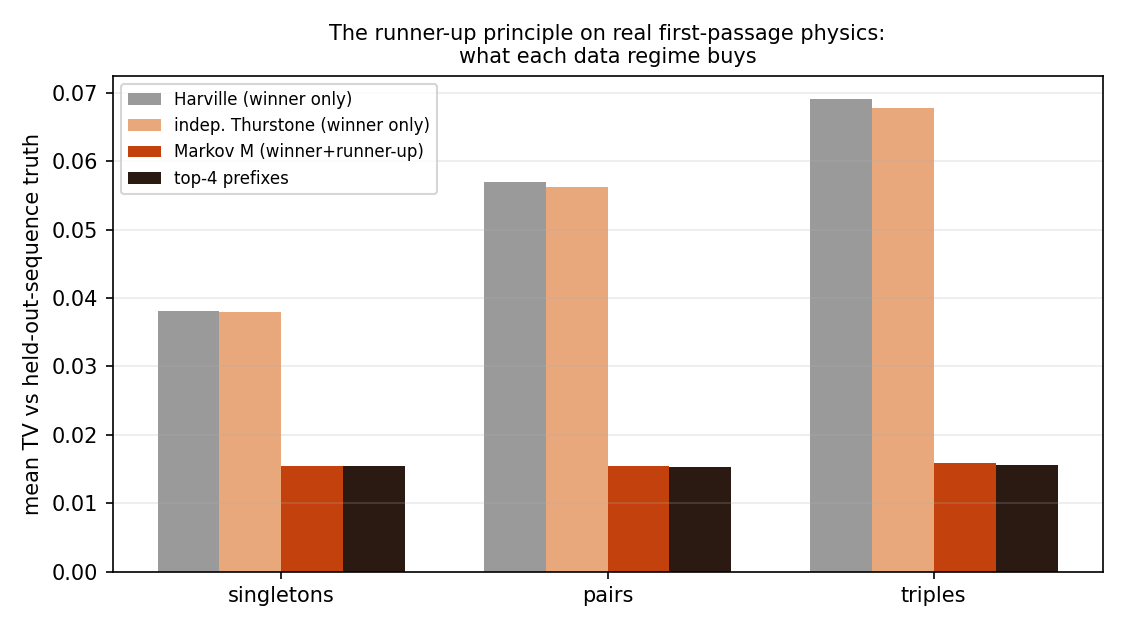
\includegraphics[width=0.82\textwidth]{figs/regimes.png}
\caption{What each data regime buys, on real first-passage physics.}
\label{fig:regimes}
\end{figure}

\section{The kernel is computable from geometry}\label{sec:geometry}

The runner-up kernel of a diffusive encounter process is a family of
first-hitting-split probabilities, and hitting splits are Green-function objects.
On a finite-volume discretization of the reflecting generator (a construction whose
invariant law, reversibility, and killed-resolvent behavior were validated
separately in experiment 9 of the repository), define
\[
p^{\mathrm{geo}}_j = \Prob_{\text{center}}(\text{first window hit is } j),
\qquad
M^{\mathrm{geo}}_{ij} = \Prob_{\partial_i}(\text{next distinct window hit is } j),
\]
both computed by sparse linear solves --- about one second for a
$10{,}560$-cell grid and $16$ windows, with no trajectory data.

Two start conventions for $M^{\mathrm{geo}}$ were compared: the invariant law
restricted to the window's boundary cells, and the \emph{exact} entry profile
(the joint law of first-window and entry cell, itself a hitting computation, making
the two-leg construction assumption-free). The refinement is a null result: it
moves the kernel by at most $0.015$ and predictions not at all. Against the
empirically measured first-transition kernel, the geometric kernel agrees to within
sampling noise: over all $240$ off-diagonal entries the largest standardized
discrepancy is $z = 4.0$, with none beyond, and the largest raw discrepancies sit
on adjacent-window entries where the discretization's ring-entry semantics blur
boundary contact by one cell depth.

\begin{table}[h]
\centering
\begin{tabular}{lccc}
\toprule
model (data consumed) & singletons & pairs & triples \\
\midrule
Harville renormalization (trajectory $p$) & 0.0369 & 0.0524 & 0.0705 \\
empirical $M$, first transitions (trajectory $p, M$) & 0.0230 & 0.0207 & 0.0208 \\
empirical $M$, all pairs (trajectory $p, M$) & 0.0240 & 0.0258 & 0.0298 \\
trajectory $p$ + geometric $M$ & \textbf{0.0221} & \textbf{0.0201} & \textbf{0.0184} \\
pure geometry ($p^{\mathrm{geo}}, M^{\mathrm{geo}}$; no trajectories) & 0.0322 & 0.0298 & 0.0277 \\
\bottomrule
\end{tabular}
\caption{Blocked-set prediction on a disjoint-window geometry (experiment 10).
The geometric kernel beats both empirical kernels at every deletion depth --- it is
noise-free and structurally consistent where empirical estimates carry sampling
noise --- and the zero-trajectory model beats winner-only \emph{trajectory} models
on pair and triple blocks. Note the two-kernels warning realized: all-pairs
estimation is strictly worse than first-transitions.}
\label{tab:exp10}
\end{table}

The conclusion we draw is stronger than ``geometry helps'': for diffusive
first-passage systems, \emph{the substitution structure is a computable geometric
object}. Winner-only observation cannot reveal it (Theorem~\ref{thm:nonid}); the
runner-up identifies it (Proposition~\ref{prop:prefix}); and where the geometry is
known, it need not be measured at all.

\section{Discussion}

Three threads lead onward. First, the objects of this paper --- the substitution
resolvent $(I - M_{BB})^{-1}$, the killed resolvent of the shared-environment race,
and the matrix inverses of harmonic defect calculations --- are one family: response
operators whose behavior under suppression and deletion is Schur-complement theory.
The companion program develops the homogenization side (softmax as the fast-mixing
limit of hidden-state races, with a Green--Kubo correction that answers every
blocked-subset counterfactual from one pair of summary objects). Second, the
practical estimation theory: sample-efficient estimation of $M$ under the
first-transition constraint, and experimental design for which interventions to
run when geometry is unknown. Third, applications where the runner-up is already
recorded but unused: exacta and trifecta markets quote the market's $M$ directly
(divide the exacta matrix by the win vector), and catalysis simulations that log
secondary reaction channels contain their own substitution kernels. In each case
the identity \eqref{eq:runnerup} converts data already collected into
counterfactuals previously assumed.

\begin{thebibliography}{9}
\bibitem{cox1959} D.~R. Cox. The analysis of exponentially distributed lifetimes
with two types of failure. \emph{JRSS-B} 21 (1959) 411--421.
\bibitem{tsiatis1975} A.~Tsiatis. A nonidentifiability aspect of the problem of
competing risks. \emph{PNAS} 72 (1975) 20--22.
\bibitem{harville1973} D.~A. Harville. Assigning probabilities to the outcomes of
multi-entry competitions. \emph{JASA} 68 (1973) 312--316.
\bibitem{luce1959} R.~D. Luce. \emph{Individual Choice Behavior}. Wiley, 1959.
\bibitem{thurstone1927} L.~L. Thurstone. A law of comparative judgment.
\emph{Psychological Review} 34 (1927) 273--286.
\bibitem{blanchet2016} J.~Blanchet, G.~Gallego, V.~Goyal. A Markov chain
approximation to choice modeling. \emph{Operations Research} 64 (2016) 886--905.
\bibitem{holcman2014} D.~Holcman, Z.~Schuss. The narrow escape problem.
\emph{SIAM Review} 56 (2014) 213--257.
\bibitem{cotton2021} P.~Cotton. Inferring relative ability from winning probability
in multientrant contests. \emph{SIAM J.\ Financial Mathematics} 12 (2021) 295--317.
\end{thebibliography}

\end{document}
